%%% %%% INITIAL COMMENTS HERE %%%
%%%
%%% Jesse Leigh Patsolic 
%%% 2023 <Jesse.L.Patsolic@alumni.wfu.edu>
%%% Tikkun Olam
%

\documentclass[25pt, a0paper, portrait, margin=0mm, innermargin=15mm,
    blockverticalspace=15mm, colspace=15mm, subcolspace=8mm]{tikzposter} %Default values for poster format options.

\usepackage{tikz}
\usetikzlibrary{calc,intersections,through,backgrounds}
\usetikzlibrary{angles}
\usetikzlibrary{automata}
\usetikzlibrary{positioning}
%\usetikzlibrary{graphs,graphdrawing,quotes}
%\usegdlibrary{routing}
\tikzposterlatexaffectionproofoff %shows small comment on how the poster was made at bottom of poster

% Commands
\newcommand{\bs}{\textbackslash}   % backslash
\newcommand{\cmd}[1]{{\bf \color{red}#1}}   % highlights command

% Title, Author, Institute
\title{Blank Poster/Slide}
%\author{Jesse L. Patsolic \sc{b.s., m.a.}}
%\institute{}

% -- PREDEFINED THEMES ---------------------- %
% Choose LAYOUT:  Default, Basic, Rays, Simple, Envelope, Wave, Board, Autumn, Desert,
\usetheme{Default}
\usecolorstyle[colorPalette=GreenGrayViolet]{Germany}

 \settitle{ \centering \vbox{
%     \@titlegraphic \\[\TP@titlegraphictotitledistance] \centering
     \color{titlefgcolor} {\bfseries \Huge \sc \@title \par}
     %\vspace*{1em}
     %{\huge \@author \par} \vspace*{1em} {\LARGE \@institute}
}}

\begin{document}

  \maketitle[width=0.80\textwidth]%[titletoblockverticalspace=10pt,titletotopverticalspace=2pt]

  \begin{columns}%blocks will be placed into columns
  \column{.50}
  \block[roundedcorners=0]{Opening Statement}{
		\begin{tikzfigure}
		\centering
			\begin{tikzpicture}[scale=5]
				\coordinate [label=left:$A$] (A) at (0,0); \coordinate [label=right:$B$] (B) at (1.25,0.25); \draw [name path=A--B] (A) -- (B);
				\node (D) [name path=D,draw,circle through=(B),label=left:$D$] at (A) {}; \node (E) [name path=E,draw,circle through=(A),label=right:$E$] at (B) {};
				\path [name intersections={of=D and E, by={[label=above:$C$]C, [label=below:$C'$]C'}}]; \draw [name path=C--C',red] (C) -- (C');
				\path [name intersections={of=A--B and C--C',by=F}];
				\node [fill=red,inner sep=1pt,label=-45:$F$] at (F) {}; 
			\end{tikzpicture}
		\end{tikzfigure}
    \innerblock[]{Inner Blocks}{
      Inner blocks may be created inside of blocks with the command \bs\texttt{innerblock[{\it options}]\{{\it Heading}\}\{{\it Text}\}} 
    }
    \coloredbox{
      Text may be highlighted using colored boxes created by \bs\texttt{coloredbox[{\it options}]\{{\it Text\}}}
    }
  }
	\block{Blocks}{
		Blocks are arranged in a grid, by default, with width by default \texttt{\bs textwdith}.

		\begin{tikzfigure}
		\centering
			
\begin{tikzpicture}[scale=5]
				\tikz \foreach \x in {1,...,10}
					\draw (\x,0) circle (0.45cm);
			\end{tikzpicture}
		\end{tikzfigure}
	}

	\column{.45}
  \block{Columns}{
		By default, blocks are arranged in a single column. If you want 
		\begin{tikzfigure}
		\centering
			\begin{tikzpicture}%[scale=5]
				\tikz \foreach \x in {1,...,10}
					\draw[ultra thick] (0,\x) circle (0.45cm);
				\tikz \foreach \x in {1,...,10}
					\draw[ultra thick] (5,\x) circle (0.45cm);
				\tikz \foreach \x in {1,...,10}
					\draw[ultra thick] (10,\x) circle (0.45cm);
			\end{tikzpicture}
		\end{tikzfigure}
  }
  \begin{subcolumns}
		\subcolumn{.45}
		\block{Subcolumns}{
			If you want to have an additional subdivision of columns inside a
			column, you may use the\\ \texttt{\bs subcolumns} environment
			inside of a column environment.  The functionality is similar to
			that of columns, but now the widths are relative to the width of
			the current column.
			}
		\subcolumn{.5}
    \block{}{
				An example use of subcolumns is 
				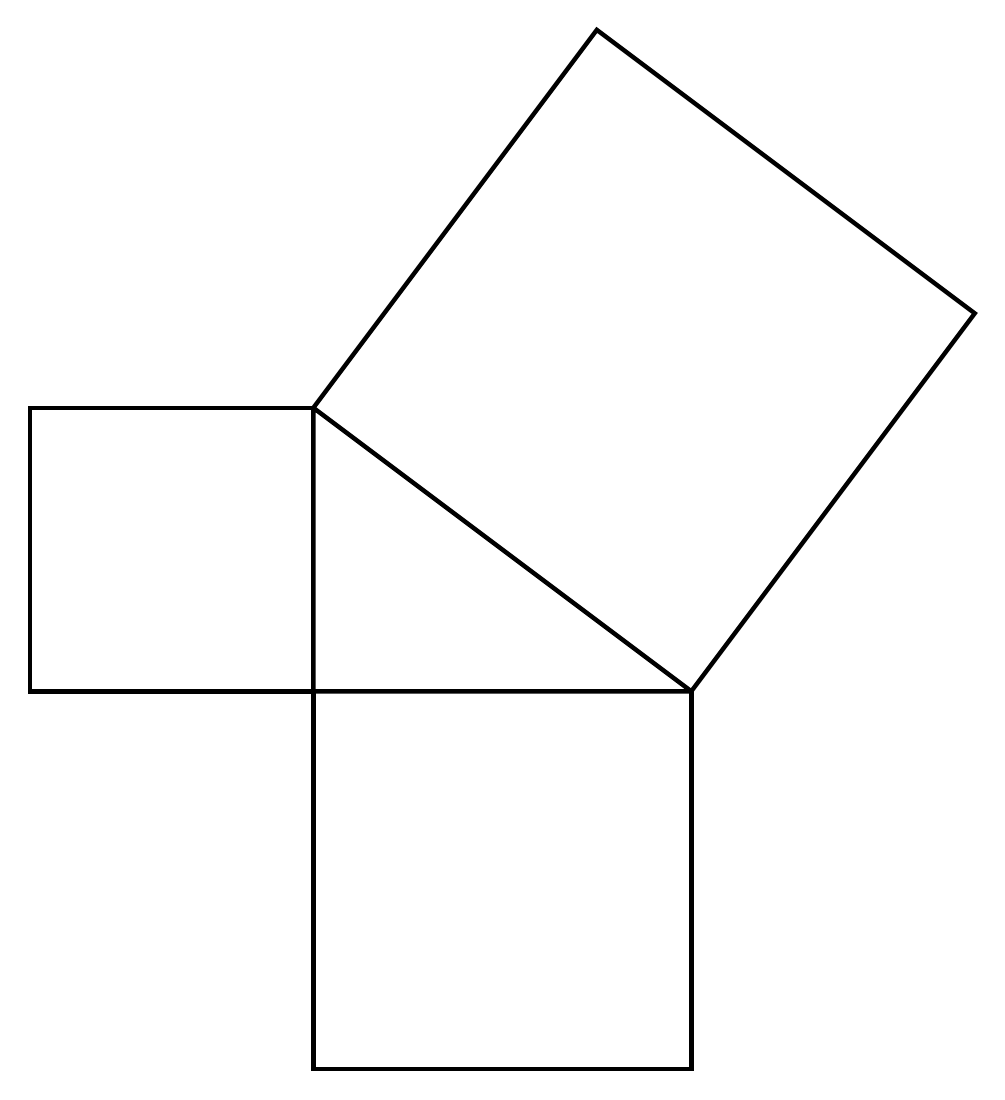
\begin{tikzpicture}[scale=1.2,ultra thick, xscale=-1]
						\draw[-, rounded corners = .5pt] (0,0) -- (4,0) -- 
								(4,3) -- (0,0);% t1
						\draw[-] (0,0) -- (0,-4) -- (4,-4) -- (4,0); % s4
						\draw[-] (4,0) -- (7,0) -- (7,3) -- (4,3); % s3
						\draw[-] (0,0) -- (-3,4) -- (1,7) -- (4,3); %
				\end{tikzpicture}
			}
	\end{subcolumns}
	\block[titlewidthscale=.8,bodywidthscale=.9,titleoffsety=9.5mm,bodyoffsety=9mm]{Changing the Poster's Appearance}{
		If the default appearance of the title, background, blocks, and
		notes is not desired, you may change the colors by calling the color
		style along with a general layout theme with the commands
		}

	\end{columns}

\end{document}


%   Time:
%%  Working status:
%%% Comments:
%%%% Tikkun Olam
